\chapter{Methods}

\section{The data}
PLease tell where is the data come from, a little brief of company can be put here.

\section{Method 1}
Definition, steps, algoritm or equation of method 1 and how to apply into your data
\section{Method 2}
Definition, steps, algoritm or equation of method 2 and how to apply into your data


\section{Aip Suprapto Munari/1164063}
\subsection{Teori}
Tugas Harian 5 
\begin{enumerate}
\item Random Forest Dan Ilustrasi Gambarnya
\begin{itemize}
\item Pengertian Random Forest:
\par Random Forest adalah suatu algoritma yang digunakan pada klasifikasi data dalam jumlah yang besar. Klasifikasi random forest dilakukan melalui penggabungan pohon  dengan melakukan training pada sampel data yang dimiliki. Penggunaan pohon (tree) yang semakin banyak akan mempengaruhi akurasi yang akan didapatkan menjadi lebih baik. Penentuan klasifikasi dengan random forest diambil berdasarkan hasil voting dari pohon yang terbentuk. Pemenang dari pohon yang terbentuk ditentukan dengan vote terbanyak. 
\par Pembangunan pohon  pada random forest sampai dengan mencapai ukuran maksimum dari pohon data. Akan tetapi,pembangunan pohon random foresttidak dilakukan pemangkasan  yang merupakan sebuah metode untuk mengurangi kompleksitas ruang.
\item Ilustrasi Gambar Random Forest :
\par

\begin{figure}[ht]
\centering
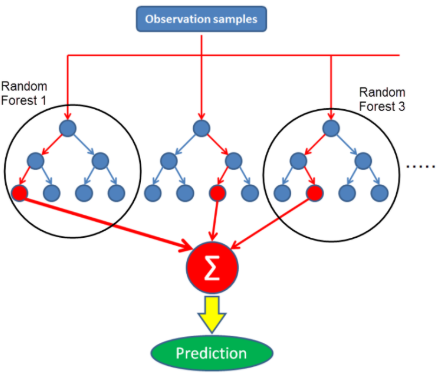
\includegraphics[scale=0.9]{figures/AIP/asm1.PNG}
\caption{Random Forest}
\label{contoh}
\end{figure}

\par
\end{itemize}

\item Cara Membaca Dataset

Berikut adalah cara membaca dataset :
\begin{itemize}
\item Buka Anaconda Navigator lalu jalankan Syder, kemudian import libraries yang dibutuhkan.
\item Masukkan kode python untuk membaca file csv, lalu jalankan

\begin{figure}[ht]
\centering
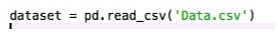
\includegraphics[scale=0.5]{figures/AIP/y1.PNG}
\caption{(b)}
\label{contoh}
\end{figure}
\par (c) Maka pada window console akan menampilkan pesan berikut :
\begin{figure}[ht]
\centering
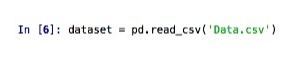
\includegraphics[scale=0.9]{figures/AIP/y2.PNG}
\caption{(c)}
\label{contoh}
\end{figure}
\par (d) Dari explorer dapat terlihat dataset yang terimport.
\begin{figure}[ht]
\centering
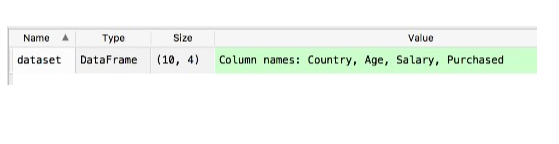
\includegraphics[scale=0.6]{figures/AIP/y3.PNG}
\caption{(d)}
\label{contoh}
\end{figure}
\par (e) Lalu klik dataset cell, maka akan muncul seperti berikut :
\begin{figure}[ht]
\centering
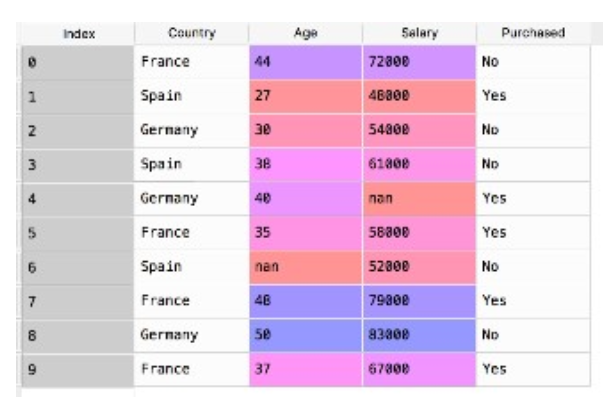
\includegraphics[scale=0.9]{figures/AIP/y4.PNG}
\caption{(e)}
\label{contoh}
\end{figure}
\par (f) Seperti yang terlihat pada gambar tersebut dataset ini memiliki Kolom Country, Age, dan Salary sebagai independent variable-nya dan kolom Purchased sebagai dependent variable-nya.
\par (g) Selanjutnya buat 2 matrix of features yang berisi values dari independent variable dan dependent variable.
\par (h) Lalu tuliskan perintah berikut :
\begin{figure}[ht]
\centering
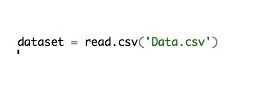
\includegraphics[scale=0.9]{figures/AIP/y5.PNG}
\caption{(h)}
\label{contoh}
\end{figure}
\par (i) Perintah yang telah dibuat di atas akan membuat sebuah global environment baru dan muncul dataset.
\par (j) Klik dataset tersebut maka muncul tabel berisi dataset.

\end{itemize}

\item Cross Validation
\begin{itemize}
\item Pengertian Cross Validation : 
\par Cross Validation adalah sebuah teknik validasi model yang digunakan untuk menilai bagaimana hasil analisis statistik akan digeneralisasi ke kumpulan data independen. Cross validation digunakan dengan tujuan prediksi, dan bila kita ingin memperkirakan seberapa akurat model model prediksi yang dilakukan dalam sebuah praktek. Tujuan dari cross validation yaitu untuk mendefinisikan dataset guna menguju dalam fase pelatihan untuk membatasi masalah seperti overfitting dan underfitting serta mendapatkan wawasan tentang bagaimana model akan digeneralisasikan ke set data independen.

\par
\end{itemize}
\item Penjelasan / Maksud Dari Score pada :
\begin{itemize}
\item Random forest ( 44\% )
\par Maksud arti score 44\%  pada random forest adalah hasil dari akurasi. Yang menggunakan 5 buah atribut yaitu dari 5 baris pertama dari set pelatihan yang akan memprediksi spesies 10, 28, 156, 10 dan 43.
\par

\item Decision Tree ( 27\% )
\par Maksud arti score 27\% pada decission tree adalah presentasi hasil dari perhitungan dataset. Dari set tentang burung pipit. Confusion matrix memberi tau hal-hal yang diharapkan, artinya, butrung-burung yang terlihat mirip saling bingung satu sama lain. 
\par

\item SVM ( 29\% )
\par Maksud arti score 29\% dari SVM adalah hasil pendekatan jaringan saraf. Di sini, akurasinya adalah 27\%, yang kurang dari akurasi 44\% sebelumnya. Oleh karena itu, dessicion tree menjadi  lebih buruk. Jika kita menggunakan Support Vector Machine (SVM), yang merupakan neural pendekatan jaringan, outputnya 29\%. Jadi 29\% pada SVM merupakan hasil otputannya.
\par
\par Hasil tersebut didapat dari hasil valdasi silang untuk memastikan bahwa membagi training test dengan cara yang berbeda. Sehingga didapat outputnya 44\% untuk hutan acak, 27\% untuk pohon keputusan, dan 29\% untuk SVM.
\par
\end{itemize}

\par
\item Confusion Matrix Dan Ilustrasinya
\begin{itemize}
\item Cara Membaca Confusion Matrix :
\par Perhitungan confusion matrix adalah sebagai berikut, akan saya beri contoh sederhana yaitu pengambilan keputusan untuk mendapatkan bantuan beasiswa. Saya menggunakan dua atribut, yaitu rekening listrik dan gaji. Yang pertama kita lakukan yaitu mencari 4 nilai yaitu a,b,c, dan d:
\par a= 4
\par b= 1
\par c= 1
\par d= 2
\par Kemudian kita dapat mencari nilai Recall, Precision, accuracy dan Error Rate
\par Recall =2/(1+2) = 0,66
\par Precision = 2/(1+2) = 0,66
\par Accuracy =(4+2)/(4+1+1+2) = 0,75
\par Error Rate =(1+1)/(4+1+1+4) = 0,2
\par Ilustrasi Confusion Matrix :
\par
\begin{figure}[ht]
\centering
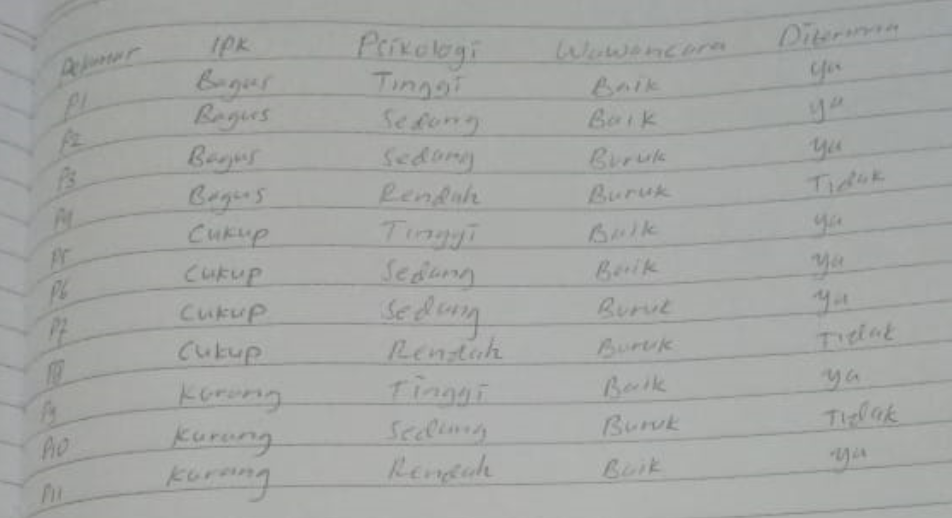
\includegraphics[scale=1]{figures/AIP/asm3.PNG}
\caption{Confussion Matrik}
\label{contoh}
\end{figure}
\end{itemize}

\par
\par
\item Voting Random Forest Dan Ilustrasi Gambarnya.
\par
\begin{itemize}
\item Pengertian Voting pada Random Forest	:
\par Metode ensemble dapat mencapai akurasi tinggi dengan membangun beberapa pengklasifikasi dan menjalankan
masing-masing secara mandiri. Ketika classifier membuat sebuah keputusan, kamu dapat memanfaatkan yang terbaik
keputusan umum dan rata-rata. Jika kita menggunakan metode yang paling umum, itu disebut voting.
\item Ilustrasi Gambar Voting Random Forest :
\begin{figure}[ht]
\centering
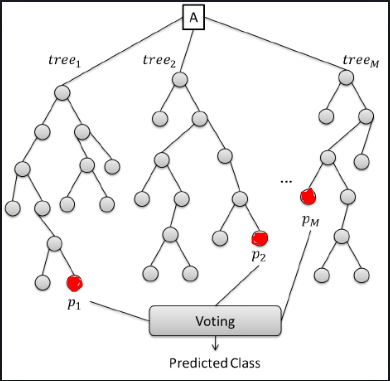
\includegraphics[scale=1]{figures/AIP/asm2.PNG}
\caption{Voting Random forest}
\label{contoh}
\end{figure}
\end{itemize}
\end{enumerate}

section{Andi Muhammad Aslam/1164064}
\begin{enumerate}

\item Random Forest merupakan algoritma yang digunakan terhadapap klasifikasi data dalam jumlah yang besar. Klasifikasi pada random forest dilakukan dengan penggabungan dicision tree dengan melakukan training terhadap sempel data yang dimiliki. Pembentukan decision tree menggunakan sample data berupa variable secara acak lalu menjalankan klasifikasi pada semua tree yang terbentuk. Random forest berupa Decision Tree agar dapat melakukan proses seleksi. Decision tree yang di buat dibagi secara strategis dari data pada kelas yang sama. Pemecahan digunakan untuk membagi data berdasarkan jenis atribut yang digunakan..  \ref{Andi}

\begin{figure}[ht]
	\centerline{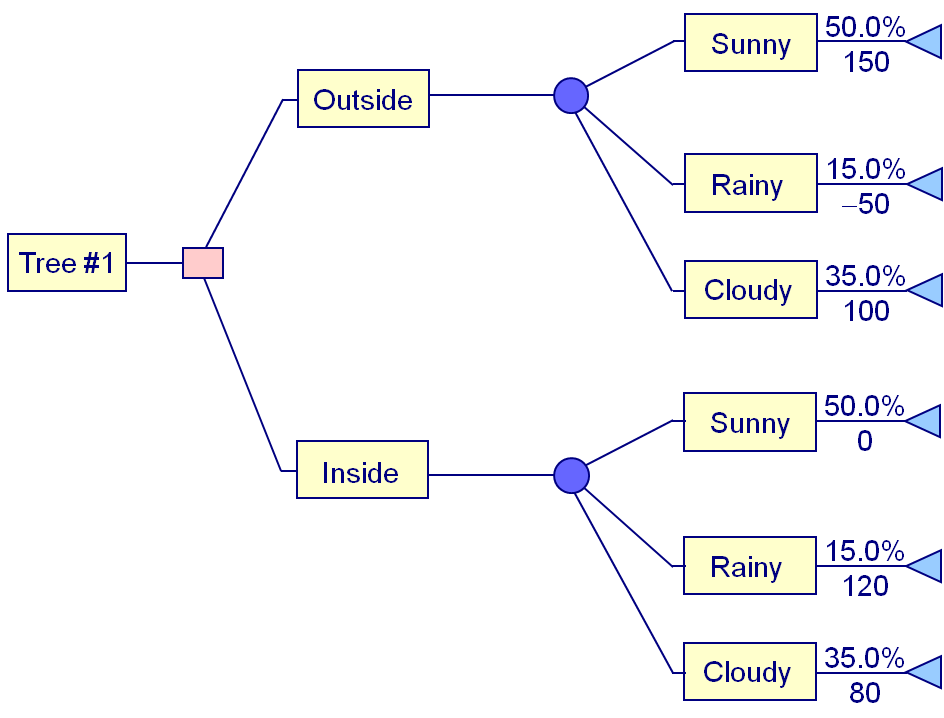
\includegraphics[width=1\textwidth]{figures/andi/decision tree.jpg}}
	\caption{Random Forest.}
	\label{contoh}
	\end{figure}

\item Download dataset terdahulu kemudian buka software spyder untuk melihat isi dataset. Data yang di download berupa extensi file bernama .txt yang terdapat class dari field. Contohnya pada data jenis burung memiliki file index dan angka, dimana index berisi angka yang memiliki makna berupa jenis burung atau bahkan nama burung sedangkan field memiliki isi nilai berupa 0 dan 1 yang dimana sifatnya boolean, Ya dan Tidak. Hal ini dikarenakan komputer hanya dapat membaca bilangan biner maka dari itu field yang di isikan berupa angka. Artinya angka 0 berarti tidak dan angka 1 berarti Ya.

\item Cross validation adalah metode statistik yang digunakan untuk memperkirakan keterampilan model pembelajaran mesin. Ini biasanya digunakan dalam pembelajaran mesin yang diterapkan untuk membandingkan dan memilih model untuk masalah pemodelan prediktif yang diberikan karena mudah dipahami, mudah diimplementasikan, dan menghasilkan estimasi keterampilan yang umumnya memiliki bias lebih rendah daripada metode lainnya.

\item Penjelasan Score
	\begin{itemize}
		\item Pada score 44\% pada random forest berupa hasil akurasi.
		\item Pada score 27\% pada decision tree adalah presentasi hasil dari perhitungan dataset.
		\item Pada  score 29\% dari SVM adalah hasil pendekatan neural network.
		\item Hasil tersebut didapat dari hasil valdasi silang untuk memastikan bahwa membagi  training test dengan cara yang berbeda. Sehingga dapat diketahui hasi output yaitu 44\% untuk hutan, 27\% untuk pohon keputusan, dan 29\% untuk SVM.
	\end{itemize}

\item Untuk membaca confusion matriks dapat menggunakan source code berikut :
	\begin{verbatim}
		import numpy as np
		np.set_printoptions(precision=2)
		plt.figure(figsize=(60,60), dpi=300)
		plot_confusion_matrix(cm, classes=birds, normalize=True)
		plt.show()
	\end{verbatim}

Dimana numpy dapat mengelola data yang berhubungan pada matrix. Pada perintah code tersebut digunakan dalam melakukan read pada dataset burung dengan menggunakan metode confusion matrix. Dalam confusion matrix memiliki 4 istilah yaitu True Positive yang merupakan data posotif yang terditeksi benar, True Negatif yang merupakan data negatif akan tetapi terditeksi benar, False Positif merupakan data negatif namun terditeksi sebagai data positif, False Negatif merupakan data posotif namun terditeksi sebagai data negatif. Adapun contoh hasil read dataset menggunakan confusion matrix dapat dilihat pada figure \ref{Andi}

\item Untuk mengetahui confusion matriks kita dapat melihat contoh klasifikasi dari biner berikut ini :
	\begin{figure}[ht]
	\centerline{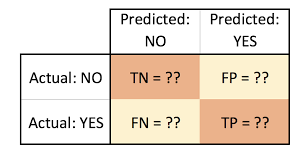
\includegraphics[width=1\textwidth]{figures/andi/CM.PNG}}
	\caption{Tabel Confusion Matriks}
	\label{contoh}
	\end{figure}
\item Voting merupakan proses pemilihan dari tree yang dimana akan dimunculkan hasilnya dan disimpulkan menjadi informasi yang pasti.
	\begin{figure}[ht]
	\centerline{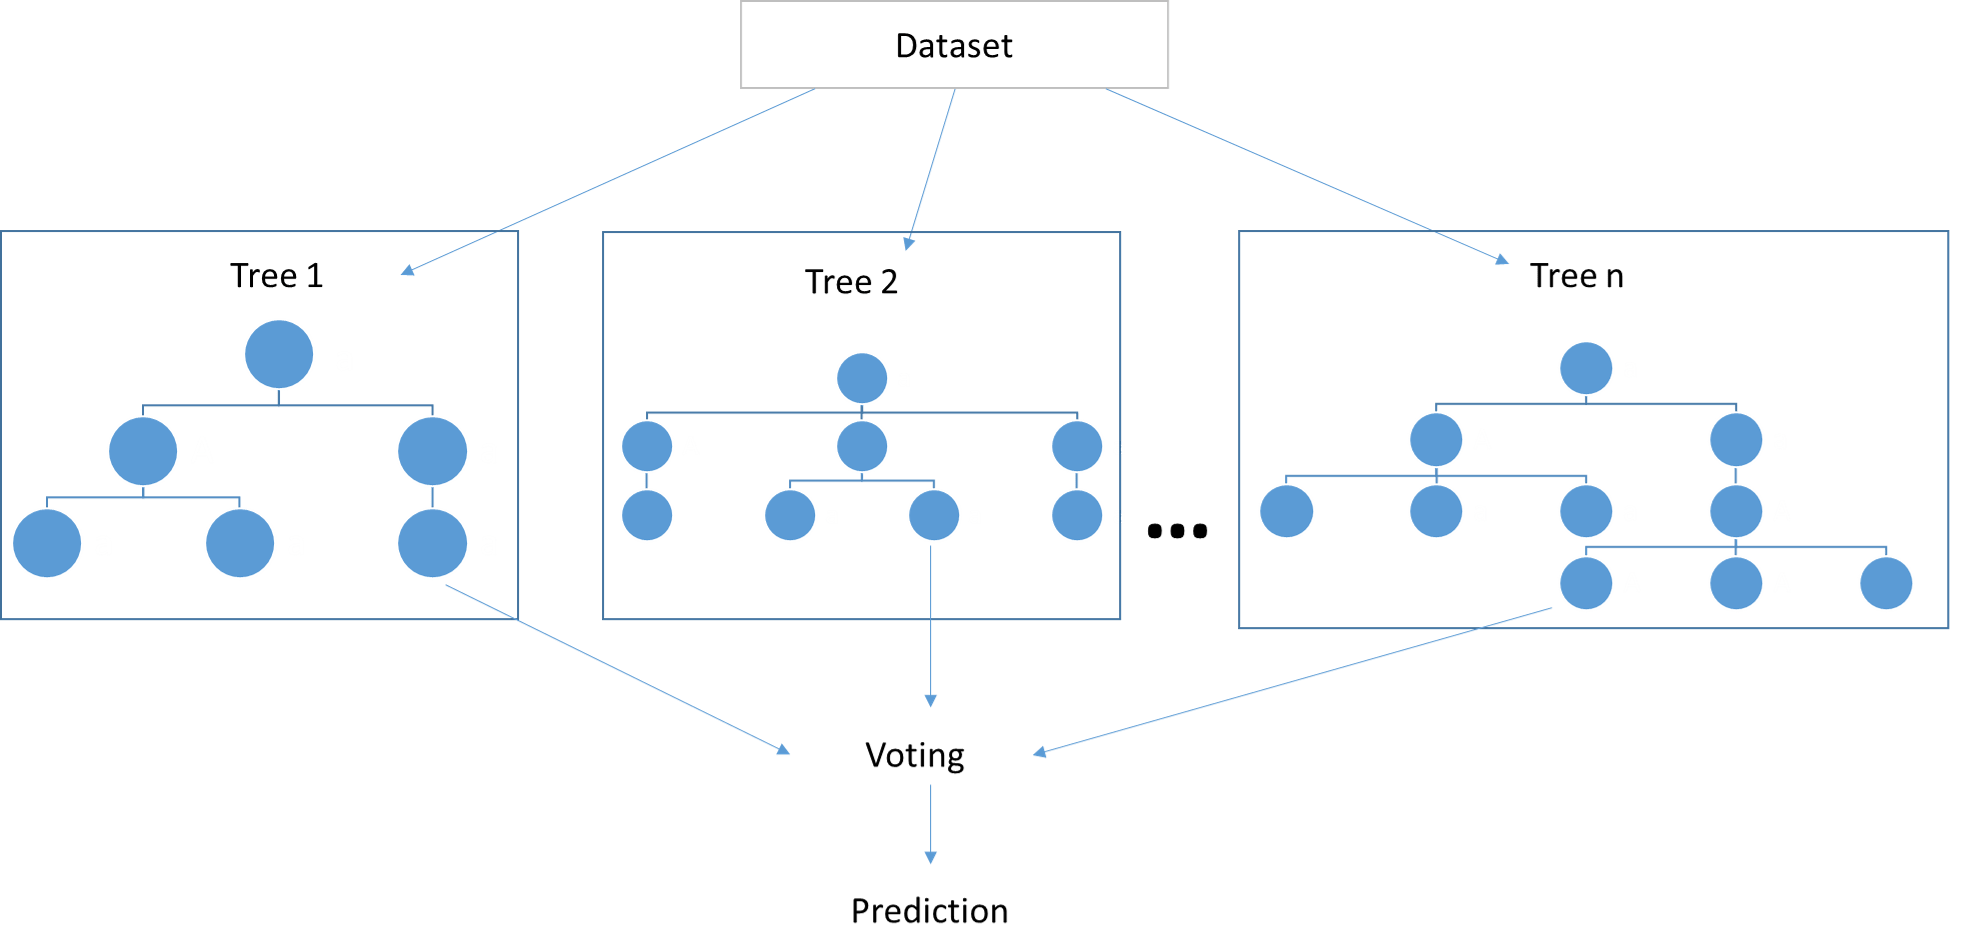
\includegraphics[width=1\textwidth]{figures/andi/Voting.PNG}}
	\caption{Voting}
	\label{Contoh Voting}
	\end{figure}

Pada figure Voting terdapat Decision Tree yang terbagi menjadi 3 Branch yaitu tree 1, tree 2, dan tree 3. Pada tree tersebut akan dilakukan proses voting. Pada  masing-masing tree tersebut memiliki data-data yang berbeda, yang di mana data tersebut akan di pilih dengan cara voting. Hasli voting dari setiap tree tersebut menunjukkan data pada setiap tree, Di sini kita dapat menghitung akurasi dengan menambahkan angka secara diagonal, sehingga ini semua adalah contoh yang diklasifikasikan dengan benar, dan membagi jumlah tersebut dengan jumlah semua angka dalam matriks.

\end{enumerate}